\documentclass{article}

\usepackage{amsmath} % Define various maths environments
\usepackage{amssymb} % Define various maths symbols
\usepackage{geometry} % Adjust the margin, paper size, and etc.
\usepackage{enumerate} % Provide different style of lists
\usepackage{graphicx} % Insert image of all types
\usepackage{xcolor}
\usepackage{ulem}
\usepackage{pdfpages}
\usepackage{array} % Provide auxiliary format for tabular
\usepackage{booktabs} % Create Three-line Table
\usepackage{bm}
\usepackage{cite}
\usepackage{url}
\usepackage{float}
\usepackage{indentfirst}
\usepackage{multirow}
\usepackage[colorlinks,linkcolor=black]{hyperref}

\begin{document}

\vspace*{0.25cm}

\noindent\hrulefill

\thispagestyle{empty}

\begin{center}
    \begin{large}
        \sc{UM--SJTU Joint Institute \vspace{0.3em} \\ Physics Laboratory \\(Vp241)}
    \end{large}

    \hrulefill

    \vspace*{5cm}
    \begin{Large}
        \sc{{Laboratory Report}}
    \end{Large}

    \vspace{2em}

    \begin{large}
        \sc{{Exercise 3
                    \vspace{0.5em}

                    Solar Cells: $I$-$V$ Characteristics}}
    \end{large}
\end{center}
\vfill

\begin{table}[h!]
    \flushleft
    \begin{tabular}{lll}
        Name: \textbf{Kang Jiaming} \hspace*{2em} &
        ID: \textbf{518021911220} \hspace*{2em}
                                                  & Group: 17 \\
        Name: Xiao Yu \hspace*{2em}               &
        ID: 518021910696 \hspace*{2em}
                                                  & Group: 17 \\
        \\

        Date: 1 Nov. 2019
    \end{tabular}
\end{table}

\hfill
\newpage
\tableofcontents
\setcounter{page}{0}
\thispagestyle{empty}
\newpage

\section{Introduction} \label{intro}

The objective of this exercise is to learn about the solar
cell and explore its characteristic ($I$-$V$, $P$-$V$, $P_{max}$, fill factor, energy conversion efficiency etc.).

Solar cells (Figure 1) are devices that transforms solar radiation into electrical energy. The principle of it is the photovoltaic effect, which is introduced in the following:

\subsection*{Photovoltaic Effect}

"When the light enters the $p$-$n$ junction near the solar cell surface, and the energy of incident photons is greater than the forbidden bandwidth (energy gap) $E_\text{g}$, the incident photons are absorbed and excite electron-hole pairs. Minority charge carriers in the $n$- or $p$-type area diffuse due to their density gradient. Some of them are able to diffuse to the region of the $p$-$n$ junction where a built-in electric field exists. This field is directed from the $n$-type to the $p$-type area. The minority carriers diffusing to the $p$-$n$ junction zone between the $n$-type area and the $p$-type area are drawn by this electric field to the $p$-type area (in case of the holes), or to the $n$-type area (in case of the electrons). This results in an increase of positive charge accumulated in the $p$-type area and negative charge in the $n$-type area. Consequently, a photoelectric potential difference is generated" [1].

\begin{figure}[H]\centering
    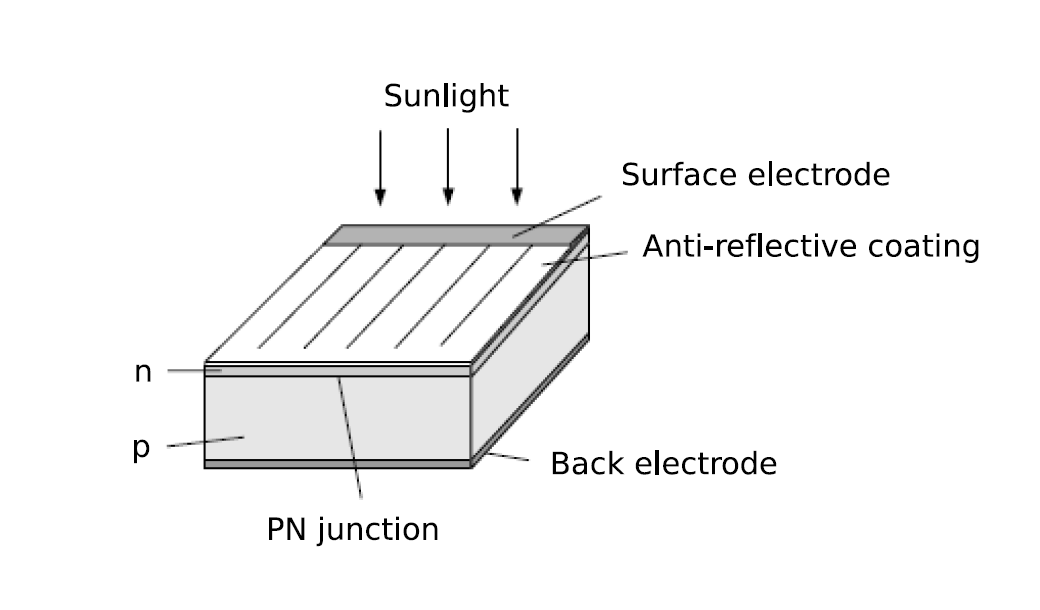
\includegraphics[scale=0.25]{pn.png}
    \caption{Structure of a crystalline silicon solar cell.}\label{FigPN}
\end{figure}

\subsection*{Solar Cell Parameters}

The open-circuit voltage $V_{oc}$ and the short-circuit current $I_{sc}$ are two basic parameters for a solar cell. Also, when there is a load resistance $R$ (with the value of $R$ ranging from zero to infinity), the corresponding $I$-$V$ values vary. If for a certain load resistance $R = R_\text{m}$ the maximum output power $P_\text{m}$ is generated, then the value of $P_\text{m}$ is
$$P_\text{m} = I_\text{m}V_\text{m},$$
where $I_\text{m}$ is called the optimal operating current, and $V_\text{m}$ is called the optimal operating voltage.

The fill factor is another important parameter of solar cells, defined as
\begin{equation}
    FF = \frac{P_\text{m}}{V_{\text{oc}}I_{\text{sc}}} = \frac{V_\text{m}I_{\text{m}}}{V_{\text{oc}}I_{\text{sc}}}.
    \label{eq:FF}
\end{equation}
Generally, the greater the fill factor is, the greater the output power.

The solar cell energy conversion efficiency $\eta$ is defined as
\begin{equation}
    \eta = \frac{P_\text{m}}{P_{\text{in}}}\times 100\%,
    \label{eq:efficiency}
\end{equation}
where $P_{\text{in}}$ denotes the total radiant power incident on the solar cell.

\section{Experimental Setup}

The experimental setup includes a photovoltaic device (5 W), a 300 W tungsten{halogen lamp
serving as a radiation source, two digital multimeters, two adjustable resistors, a solar
power meter, a wiring board and a measuring tape.

The precision of the devices used is shown in Table 1.

\begin{table}[H]
    \centering
    \begin{tabular}{cc}
        \toprule
        Quantity    & Precision           \\
        \midrule
        DC voltage  & $0.5\% + 0.01$ [V]  \\
        DC current  & $1.5\% + 0.1$ [mA]  \\
        Distance    & 0.1 [cm]            \\
        Solar power & 10 [$\text{W/m}^2$] \\
        \bottomrule
    \end{tabular}
    \caption{Precision of the measurement instruments.}\label{tablePresicion}
\end{table}

\section{Measurement Procedure}
In this experiment, the characteristic of four configurations of the solar cell are studied. For each configuration, the $I$-$V$, $P$-$V$, $P$-$R$ relation are studied and for the single configurations, the information about fill factor and energy conversion efficiency are also explored.
\begin{enumerate}
    \item First, the characteristics of two devices in series and in parallel are explored. The two devices are adjusted so that they are of the same $V_{oc}$ and $I_{sc}$. Connect the measurement circuit. Then adjust the resistance connected so that enough data of $V$ and $I$ are obtained.
    \item Then, repeat the first step for a single device, with the distance maintained the same.
    \item Measure the power on the surface of the solar board.
    \item Measure the area of the solar board.
    \item  Change the distance, repeat the first step, still for a single device.
\end{enumerate}

\subsection*{Caution}
\begin{enumerate}
    \item Do \textbf{NOT} touch the cover of the light source in case of getting burnt.
    \item Beware of the high voltage supply of the light source.
    \item Keep the distance from step 1 to 4.
    \item Do \textbf{NOT} move around so as to maintain a constant incident power.
\end{enumerate}

\section{Results}

\subsection{$I$-$V$ Relation}

The measurement data for $U$ and $I$ under different conditions are shown in Table 2 and 3.

\begin{table}[H]
    \centering
    \begin{tabular}{ccc||cc}
        \toprule
           & \multicolumn{2}{c||}{Series} & \multicolumn{2}{c}{Parallel}                                        \\
        \midrule
           & $V$ [V]                      & $I$ [mA]                     & $V$ [V]           & $I$ [mA]         \\
        \midrule
        1  & 0.84    $\pm$ 0.01           & 39.1    $\pm$ 0.7            & 1.10   $\pm$ 0.02 & 78.6   $\pm$ 1.3 \\
        2  & 1.81    $\pm$ 0.02           & 38.6    $\pm$ 0.7            & 1.75   $\pm$ 0.02 & 77.0   $\pm$ 1.3 \\
        3  & 2.72    $\pm$ 0.02           & 38.1    $\pm$ 0.7            & 2.56   $\pm$ 0.02 & 75.0   $\pm$ 1.2 \\
        4  & 3.72    $\pm$ 0.03           & 37.6    $\pm$ 0.7            & 3.38   $\pm$ 0.03 & 73.1   $\pm$ 1.2 \\
        5  & 4.82    $\pm$ 0.03           & 36.9    $\pm$ 0.7            & 4.06   $\pm$ 0.03 & 71.3   $\pm$ 1.2 \\
        6  & 6.04    $\pm$ 0.04           & 36.1    $\pm$ 0.6            & 4.58   $\pm$ 0.03 & 69.7   $\pm$ 1.1 \\
        7  & 6.94    $\pm$ 0.04           & 35.6    $\pm$ 0.6            & 4.92   $\pm$ 0.03 & 68.2   $\pm$ 1.1 \\
        8  & 7.74    $\pm$ 0.05           & 35.1    $\pm$ 0.6            & 5.12   $\pm$ 0.04 & 67.5   $\pm$ 1.1 \\
        9  & 8.82    $\pm$ 0.05           & 34.3    $\pm$ 0.6            & 5.26   $\pm$ 0.04 & 66.3   $\pm$ 1.1 \\
        10 & 9.90    $\pm$ 0.06           & 33.4    $\pm$ 0.6            & 5.39   $\pm$ 0.04 & 65.6   $\pm$ 1.1 \\
        11 & 11.08   $\pm$ 0.07           & 32.0    $\pm$ 0.6            & 5.50   $\pm$ 0.04 & 64.8   $\pm$ 1.1 \\
        12 & 11.34   $\pm$ 0.07           & 31.4    $\pm$ 0.6            & 5.78   $\pm$ 0.04 & 62.6   $\pm$ 1.0 \\
        13 & 11.59   $\pm$ 0.07           & 31.0    $\pm$ 0.6            & 5.95   $\pm$ 0.04 & 61.4   $\pm$ 1.0 \\
        14 & 11.85   $\pm$ 0.07           & 30.7    $\pm$ 0.6            & 6.04   $\pm$ 0.04 & 60.5   $\pm$ 1.0 \\
        15 & 12.29   $\pm$ 0.07           & 29.7    $\pm$ 0.5            & 6.12   $\pm$ 0.04 & 59.8   $\pm$ 1.0 \\
        16 & 12.50   $\pm$ 0.07           & 29.2    $\pm$ 0.5            & 6.23   $\pm$ 0.04 & 58.6   $\pm$ 1.0 \\
        17 & 12.76   $\pm$ 0.07           & 28.6    $\pm$ 0.5            & 6.32   $\pm$ 0.04 & 57.9   $\pm$ 1.0 \\
        18 & 13.13   $\pm$ 0.08           & 27.7    $\pm$ 0.5            & 6.72   $\pm$ 0.04 & 53.7   $\pm$ 0.9 \\
        19 & 13.45   $\pm$ 0.08           & 26.7    $\pm$ 0.5            & 7.06   $\pm$ 0.05 & 48.8   $\pm$ 0.8 \\
        20 & 13.85   $\pm$ 0.08           & 25.4    $\pm$ 0.5            & 7.41   $\pm$ 0.05 & 42.8   $\pm$ 0.7 \\
        21 & 14.28   $\pm$ 0.08           & 23.9    $\pm$ 0.5            & 7.74   $\pm$ 0.05 & 35.7   $\pm$ 0.6 \\
        22 & 14.68   $\pm$ 0.08           & 22.1    $\pm$ 0.4            & 8.06   $\pm$ 0.05 & 27.4   $\pm$ 0.5 \\
        23 & 15.08   $\pm$ 0.09           & 20.2    $\pm$ 0.4            & 8.33   $\pm$ 0.05 & 19.1   $\pm$ 0.4 \\
        24 & 15.46   $\pm$ 0.09           & 18.1    $\pm$ 0.4            & 8.57   $\pm$ 0.05 & 10.2   $\pm$ 0.3 \\
        25 & 15.83   $\pm$ 0.09           & 15.9    $\pm$ 0.3            & 8.61   $\pm$ 0.05 & 8.7    $\pm$ 0.2 \\
        \bottomrule
    \end{tabular}
    \caption{Measurement data for the $U$ vs. $I$ relation (series/parallel configuration).}\label{TableUISP}
\end{table}

\begin{table}[H]
    \centering
    \begin{tabular}{ccc||cc}
        \toprule
           & \multicolumn{2}{c||}{197.5 cm} & \multicolumn{2}{c}{165.6 cm}                                      \\
        \midrule
           & $V$ [V]                        & $I$ [mA]                     & $V$ [V]          & $I$ [mA]        \\
        \midrule
        1  & 1.14  $\pm$ 0.02               & 36.4  $\pm$ 0.6              & 1.09  $\pm$ 0.02 & 52.0  $\pm$ 0.9 \\
        2  & 1.74  $\pm$ 0.02               & 35.9  $\pm$ 0.6              & 1.73  $\pm$ 0.02 & 51.6  $\pm$ 0.9 \\
        3  & 2.65  $\pm$ 0.02               & 35.0  $\pm$ 0.6              & 2.57  $\pm$ 0.02 & 50.6  $\pm$ 0.9 \\
        4  & 3.35  $\pm$ 0.03               & 34.4  $\pm$ 0.6              & 3.23  $\pm$ 0.03 & 49.6  $\pm$ 0.8 \\
        5  & 4.11  $\pm$ 0.03               & 33.6  $\pm$ 0.6              & 3.88  $\pm$ 0.03 & 48.4  $\pm$ 0.8 \\
        6  & 4.65  $\pm$ 0.03               & 32.9  $\pm$ 0.6              & 4.52  $\pm$ 0.03 & 47.4  $\pm$ 0.8 \\
        7  & 4.93  $\pm$ 0.03               & 32.6  $\pm$ 0.6              & 5.11  $\pm$ 0.04 & 46.3  $\pm$ 0.8 \\
        8  & 5.09  $\pm$ 0.04               & 32.0  $\pm$ 0.6              & 5.40  $\pm$ 0.04 & 45.6  $\pm$ 0.8 \\
        9  & 5.33  $\pm$ 0.04               & 31.7  $\pm$ 0.6              & 5.71  $\pm$ 0.04 & 45.0  $\pm$ 0.8 \\
        10 & 5.72  $\pm$ 0.04               & 30.6  $\pm$ 0.6              & 5.92  $\pm$ 0.04 & 44.6  $\pm$ 0.8 \\
        11 & 5.91  $\pm$ 0.04               & 29.9  $\pm$ 0.5              & 6.04  $\pm$ 0.04 & 44.3  $\pm$ 0.8 \\
        12 & 6.01  $\pm$ 0.04               & 29.4  $\pm$ 0.5              & 6.19  $\pm$ 0.04 & 43.8  $\pm$ 0.8 \\
        13 & 6.06  $\pm$ 0.04               & 29.3  $\pm$ 0.5              & 6.32  $\pm$ 0.04 & 43.6  $\pm$ 0.8 \\
        14 & 6.11  $\pm$ 0.04               & 29.1  $\pm$ 0.5              & 6.45  $\pm$ 0.04 & 42.8  $\pm$ 0.7 \\
        15 & 6.16  $\pm$ 0.04               & 28.7  $\pm$ 0.5              & 6.54  $\pm$ 0.04 & 42.4  $\pm$ 0.7 \\
        16 & 6.21  $\pm$ 0.04               & 28.5  $\pm$ 0.5              & 6.66  $\pm$ 0.04 & 41.9  $\pm$ 0.7 \\
        17 & 6.31  $\pm$ 0.04               & 28.1  $\pm$ 0.5              & 6.72  $\pm$ 0.04 & 41.6  $\pm$ 0.7 \\
        18 & 6.50  $\pm$ 0.04               & 27.1  $\pm$ 0.5              & 6.76  $\pm$ 0.04 & 41.4  $\pm$ 0.7 \\
        19 & 6.73  $\pm$ 0.04               & 25.7  $\pm$ 0.5              & 6.90  $\pm$ 0.04 & 40.2  $\pm$ 0.7 \\
        20 & 7.02  $\pm$ 0.05               & 23.8  $\pm$ 0.5              & 7.15  $\pm$ 0.05 & 38.5  $\pm$ 0.7 \\
        21 & 7.36  $\pm$ 0.05               & 20.8  $\pm$ 0.4              & 7.44  $\pm$ 0.05 & 36.0  $\pm$ 0.6 \\
        22 & 7.73  $\pm$ 0.05               & 17.2  $\pm$ 0.4              & 7.73  $\pm$ 0.05 & 32.9  $\pm$ 0.6 \\
        23 & 7.91  $\pm$ 0.05               & 14.6  $\pm$ 0.3              & 8.18  $\pm$ 0.05 & 26.7  $\pm$ 0.5 \\
        24 & 8.09  $\pm$ 0.05               & 12.5  $\pm$ 0.3              & 8.78  $\pm$ 0.05 & 15.3  $\pm$ 0.3 \\
        25 & 8.34  $\pm$ 0.05               & 8.4   $\pm$ 0.2              & 9.01  $\pm$ 0.06 & 9.1   $\pm$ 0.2 \\
        \bottomrule
    \end{tabular}
    \caption{Measurement data for the $U$ vs. $I$ relation (197.5 cm/165.6 cm configuration).}\label{TableUI100}
\end{table}

The $I$-$V$ characteristic curves of the four configurations are plotted using Originlab. The plots are presented in Figure 2.

\begin{figure}[H]\centering
    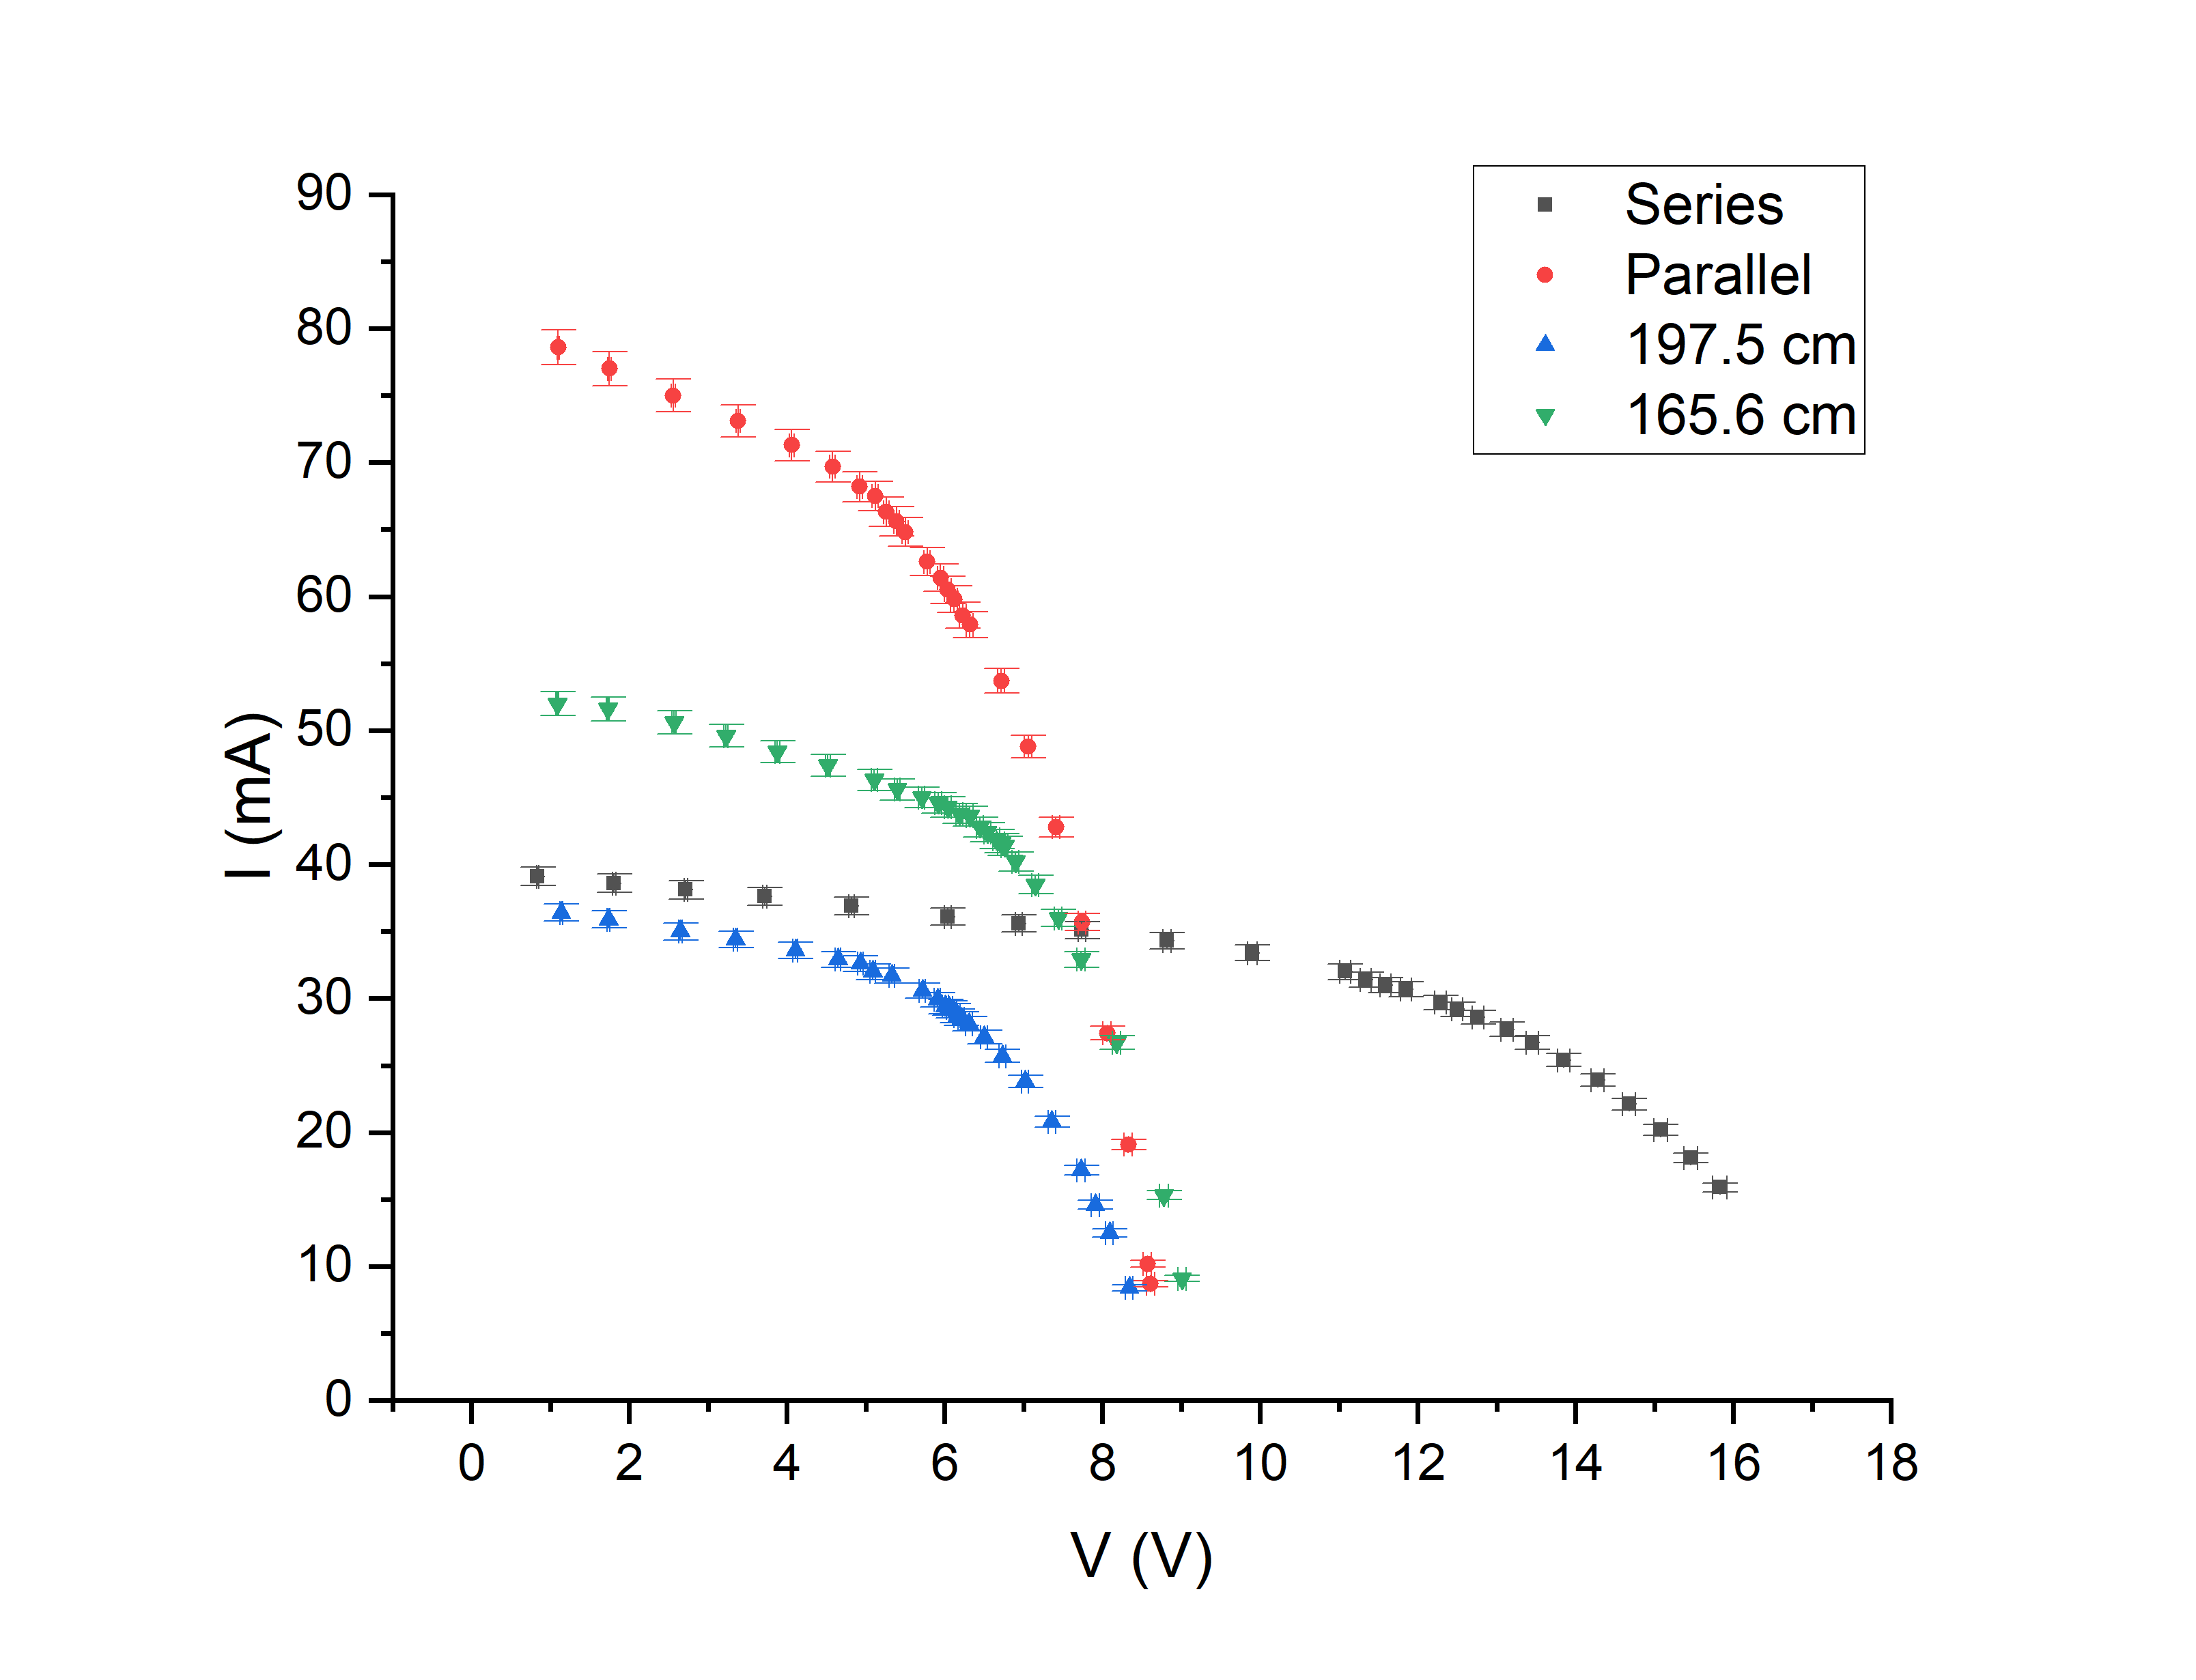
\includegraphics[scale=0.4]{I_V.png}
    \caption{$I$-$V$ characteristic curves of each configuration.}\label{FigI_V}
\end{figure}

\subsection{$P$-$V$ and $P$-$R$ Relation}

The power of the solar cell is calculated as the product of $V$ and $I$. Take the first set of data as an example,
$$P = VI = 0.84 \times 39.1 \times 10^{-3} = 0.0328 \pm 0.0008\,\,\text{W}.$$

The resistance of the external load are caluclated through Ohm's law $\displaystyle R = \frac{V}{I}$. Take the first set of data as an example,
$$R = \frac{V}{I} = \frac{0.84}{39.1\times 10^{-3}} = 21.5 \pm 0.5\,\,\Omega.$$

Perform simialr calculation for each set of data, the results are presented in Table 4 and Table 5.

\begin{table}
    \centering
    \begin{tabular}{ccc||cc}
        \toprule
           & \multicolumn{2}{c||}{Series} & \multicolumn{2}{c}{Parallel}                                                      \\
        \midrule
           & $P$ [W]                      & $R$ [$\Omega$]                & $P$ [W]             & $R$ [$\Omega$]              \\
        \midrule
        1  & 0.0328 $\pm$ 0.0008          & 21.5                $\pm$ 0.5 & 0.0865 $\pm$ 0.0019 & 14.0              $\pm$ 0.3 \\
        2  & 0.069  $\pm$ 0.0014          & 46.9                $\pm$ 1.0 & 0.135  $\pm$ 0.003  & 22.7              $\pm$ 0.4 \\
        3  & 0.104  $\pm$ 0.002           & 71.4                $\pm$ 1.4 & 0.192  $\pm$ 0.004  & 34.1              $\pm$ 0.6 \\
        4  & 0.140  $\pm$ 0.003           & 98.9                $\pm$ 1.9 & 0.247  $\pm$ 0.004  & 46.2              $\pm$ 0.8 \\
        5  & 0.178  $\pm$ 0.003           & 131                 $\pm$ 2   & 0.289  $\pm$ 0.005  & 56.9              $\pm$ 1.0 \\
        6  & 0.218  $\pm$ 0.004           & 167                 $\pm$ 3   & 0.319  $\pm$ 0.006  & 65.7              $\pm$ 1.2 \\
        7  & 0.247  $\pm$ 0.005           & 195                 $\pm$ 4   & 0.336  $\pm$ 0.006  & 72.1              $\pm$ 1.3 \\
        8  & 0.272  $\pm$ 0.005           & 221                 $\pm$ 4   & 0.346  $\pm$ 0.006  & 75.9              $\pm$ 1.4 \\
        9  & 0.303  $\pm$ 0.006           & 257                 $\pm$ 5   & 0.349  $\pm$ 0.006  & 79.3              $\pm$ 1.4 \\
        10 & 0.331  $\pm$ 0.006           & 296                 $\pm$ 6   & 0.354  $\pm$ 0.006  & 82.2              $\pm$ 1.5 \\
        11 & 0.355  $\pm$ 0.007           & 346                 $\pm$ 7   & 0.356  $\pm$ 0.006  & 84.9              $\pm$ 1.5 \\
        12 & 0.356  $\pm$ 0.007           & 361                 $\pm$ 7   & 0.362  $\pm$ 0.006  & 92.3              $\pm$ 1.7 \\
        13 & 0.359  $\pm$ 0.007           & 374                 $\pm$ 7   & 0.365  $\pm$ 0.007  & 96.9              $\pm$ 1.7 \\
        14 & 0.364  $\pm$ 0.007           & 386                 $\pm$ 7   & 0.365  $\pm$ 0.007  & 99.8              $\pm$ 1.8 \\
        15 & 0.365  $\pm$ 0.007           & 414                 $\pm$ 8   & 0.366  $\pm$ 0.007  & 102.3             $\pm$ 1.8 \\
        16 & 0.365  $\pm$ 0.007           & 428                 $\pm$ 8   & 0.365  $\pm$ 0.007  & 106.3             $\pm$ 1.9 \\
        17 & 0.365  $\pm$ 0.007           & 446                 $\pm$ 9   & 0.366  $\pm$ 0.007  & 109.2             $\pm$ 2.0 \\
        18 & 0.364  $\pm$ 0.007           & 474                 $\pm$ 9   & 0.361  $\pm$ 0.007  & 125               $\pm$ 2   \\
        19 & 0.359  $\pm$ 0.007           & 504                 $\pm$ 10  & 0.345  $\pm$ 0.006  & 145               $\pm$ 3   \\
        20 & 0.352  $\pm$ 0.007           & 545                 $\pm$ 11  & 0.317  $\pm$ 0.006  & 173               $\pm$ 3   \\
        21 & 0.341  $\pm$ 0.007           & 597                 $\pm$ 12  & 0.276  $\pm$ 0.005  & 217               $\pm$ 4   \\
        22 & 0.324  $\pm$ 0.007           & 664                 $\pm$ 14  & 0.221  $\pm$ 0.004  & 294               $\pm$ 6   \\
        23 & 0.305  $\pm$ 0.006           & 747                 $\pm$ 15  & 0.159  $\pm$ 0.003  & 436               $\pm$ 9   \\
        24 & 0.280  $\pm$ 0.006           & 854                 $\pm$ 18  & 0.087  $\pm$ 0.002  & $(84\pm 2)\times 10^{1}$    \\
        25 & 0.252  $\pm$ 0.006           & $(100\pm 2)\times 10^{1}$     & 0.075  $\pm$ 0.002  & $(99\pm 2)\times 10^{1}$    \\
        \bottomrule
    \end{tabular}
    \caption{Power $P$ and resistance $R$ for the series/parallel configuration.}
    \label{tab:PRsingle}
\end{table}

\begin{table}[H]\centering
    \begin{tabular}{ccc||cc}
        \toprule
           & \multicolumn{2}{c||}{197.5 cm} & \multicolumn{2}{c}{165.5 cm}                                                       \\
        \midrule
           & $P$ [W]                        & $R$ [$\Omega$]               & $P$ [W]              & $R$ [$\Omega$]               \\
        \midrule
        1  & 0.0415  $\pm$ 0.0009           & 31.3               $\pm$ 0.7 & 0.0567  $\pm$ 0.0013 & 21.0               $\pm$ 0.5 \\
        2  & 0.0625  $\pm$ 0.0013           & 48.5               $\pm$ 1.0 & 0.0893  $\pm$ 0.0018 & 33.5               $\pm$ 0.7 \\
        3  & 0.0928  $\pm$ 0.0018           & 75.7               $\pm$ 1.5 & 0.130   $\pm$ 0.002  & 50.8               $\pm$ 1.0 \\
        4  & 0.115   $\pm$ 0.002            & 97.4               $\pm$ 1.9 & 0.160   $\pm$ 0.003  & 65.1               $\pm$ 1.2 \\
        5  & 0.138   $\pm$ 0.003            & 122                $\pm$ 2   & 0.188   $\pm$ 0.004  & 80.2               $\pm$ 1.5 \\
        6  & 0.153   $\pm$ 0.003            & 141                $\pm$ 3   & 0.214   $\pm$ 0.004  & 95.4               $\pm$ 1.8 \\
        7  & 0.161   $\pm$ 0.003            & 151                $\pm$ 3   & 0.237   $\pm$ 0.004  & 110                $\pm$ 2   \\
        8  & 0.163   $\pm$ 0.003            & 159                $\pm$ 3   & 0.246   $\pm$ 0.005  & 118                $\pm$ 2   \\
        9  & 0.169   $\pm$ 0.003            & 168                $\pm$ 3   & 0.257   $\pm$ 0.005  & 127                $\pm$ 2   \\
        10 & 0.175   $\pm$ 0.003            & 187                $\pm$ 4   & 0.264   $\pm$ 0.005  & 133                $\pm$ 2   \\
        11 & 0.177   $\pm$ 0.003            & 198                $\pm$ 4   & 0.268   $\pm$ 0.005  & 136                $\pm$ 3   \\
        12 & 0.177   $\pm$ 0.003            & 204                $\pm$ 4   & 0.271   $\pm$ 0.005  & 141                $\pm$ 3   \\
        13 & 0.178   $\pm$ 0.003            & 207                $\pm$ 4   & 0.276   $\pm$ 0.005  & 145                $\pm$ 3   \\
        14 & 0.178   $\pm$ 0.003            & 210                $\pm$ 4   & 0.276   $\pm$ 0.005  & 151                $\pm$ 3   \\
        15 & 0.177   $\pm$ 0.003            & 215                $\pm$ 4   & 0.277   $\pm$ 0.005  & 154                $\pm$ 3   \\
        16 & 0.177   $\pm$ 0.003            & 218                $\pm$ 4   & 0.279   $\pm$ 0.005  & 159                $\pm$ 3   \\
        17 & 0.177   $\pm$ 0.003            & 225                $\pm$ 4   & 0.280   $\pm$ 0.005  & 162                $\pm$ 3   \\
        18 & 0.176   $\pm$ 0.003            & 240                $\pm$ 5   & 0.280   $\pm$ 0.005  & 163                $\pm$ 3   \\
        19 & 0.173   $\pm$ 0.003            & 262                $\pm$ 5   & 0.277   $\pm$ 0.005  & 172                $\pm$ 3   \\
        20 & 0.167   $\pm$ 0.003            & 295                $\pm$ 6   & 0.275   $\pm$ 0.005  & 186                $\pm$ 3   \\
        21 & 0.153   $\pm$ 0.003            & 354                $\pm$ 7   & 0.268   $\pm$ 0.005  & 207                $\pm$ 4   \\
        22 & 0.133   $\pm$ 0.003            & 449                $\pm$ 10  & 0.254   $\pm$ 0.005  & 235                $\pm$ 4   \\
        23 & 0.115   $\pm$ 0.003            & 542                $\pm$ 12  & 0.218   $\pm$ 0.004  & 306                $\pm$ 6   \\
        24 & 0.101   $\pm$ 0.002            & 647                $\pm$ 15  & 0.134   $\pm$ 0.003  & 574                $\pm$ 13  \\
        25 & 0.0701  $\pm$ 0.0019           & $(99\pm 2)\times 10^{1}$     & 0.082   $\pm$ 0.002  & $(99\pm 2)\times 10^{1}$     \\
        \bottomrule
    \end{tabular}
    \caption{Power $P$ and resistance $R$ for the 197.5 cm/165.6 cm configuration.}\label{TablePRSP}
\end{table}

The $P$-$V$ and $P$-$R$ characteristic curves of the four configurations are plotted using Originlab. The plots are presented in Figure 3 and 4.

\begin{figure}[H]\centering
    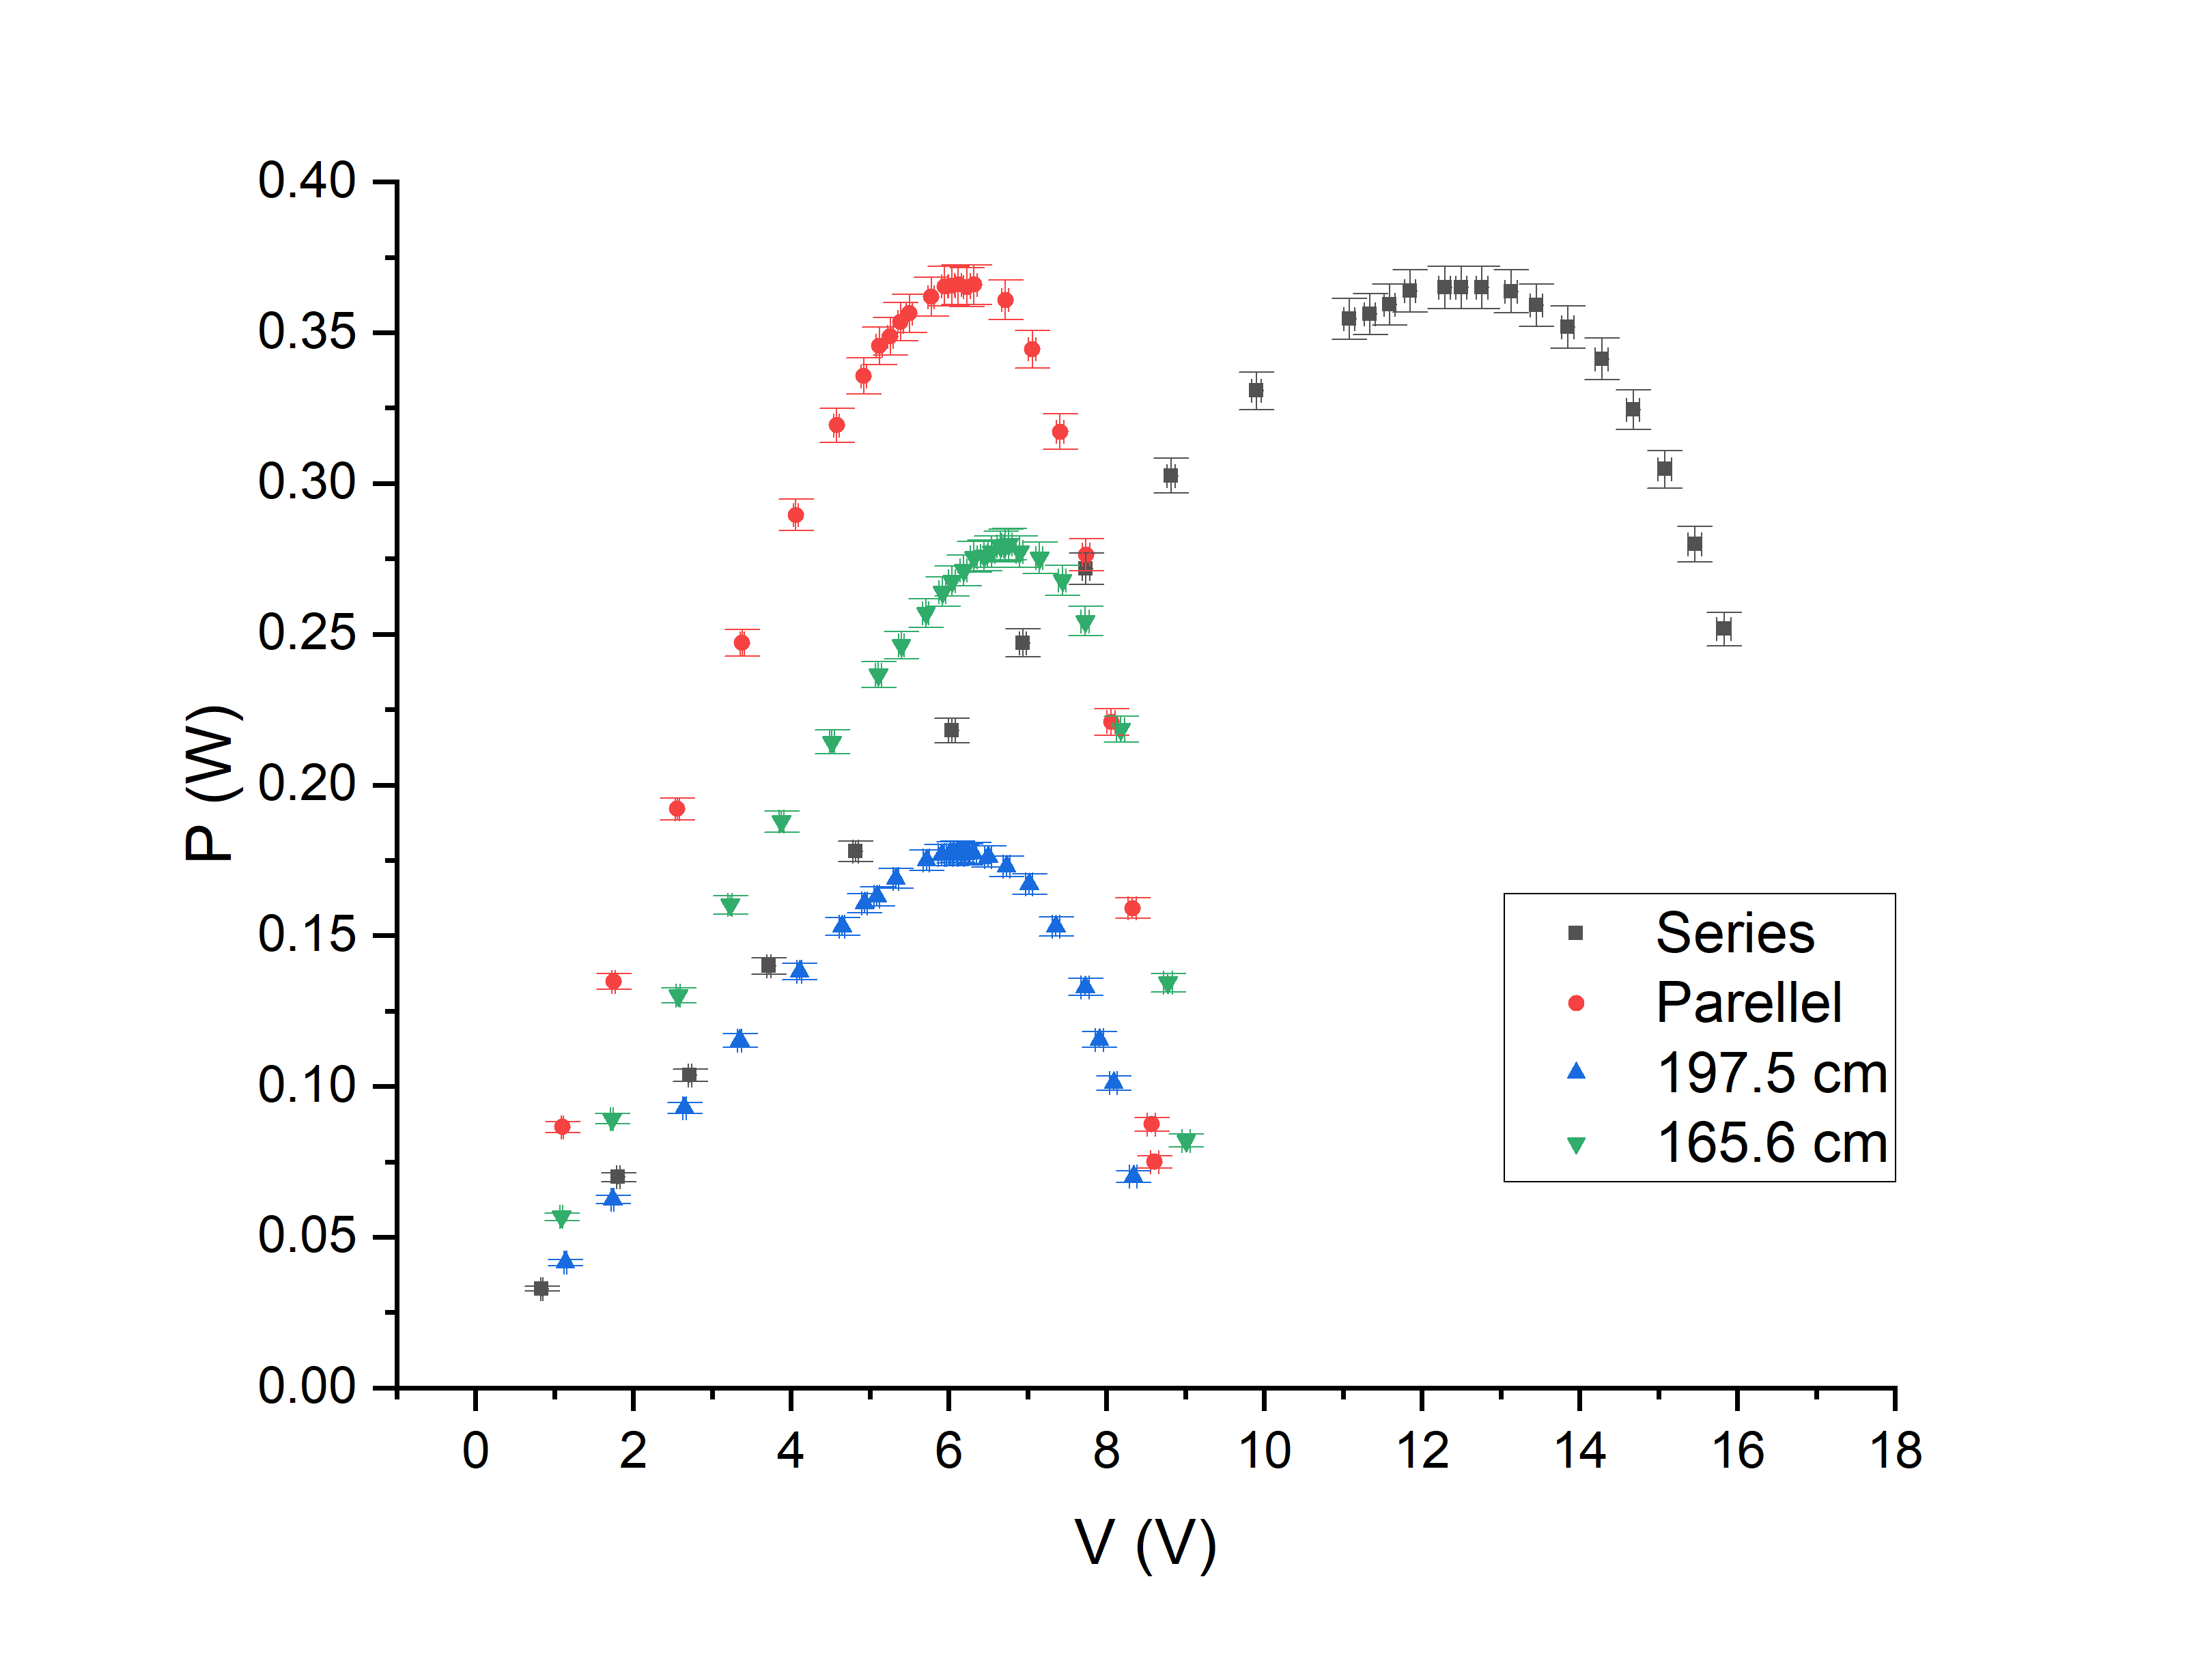
\includegraphics[scale=0.4]{P.png}
    \caption{$P$-$V$ characteristic curves of each configuration.}\label{FigP}
\end{figure}



\begin{figure}[H]\centering
    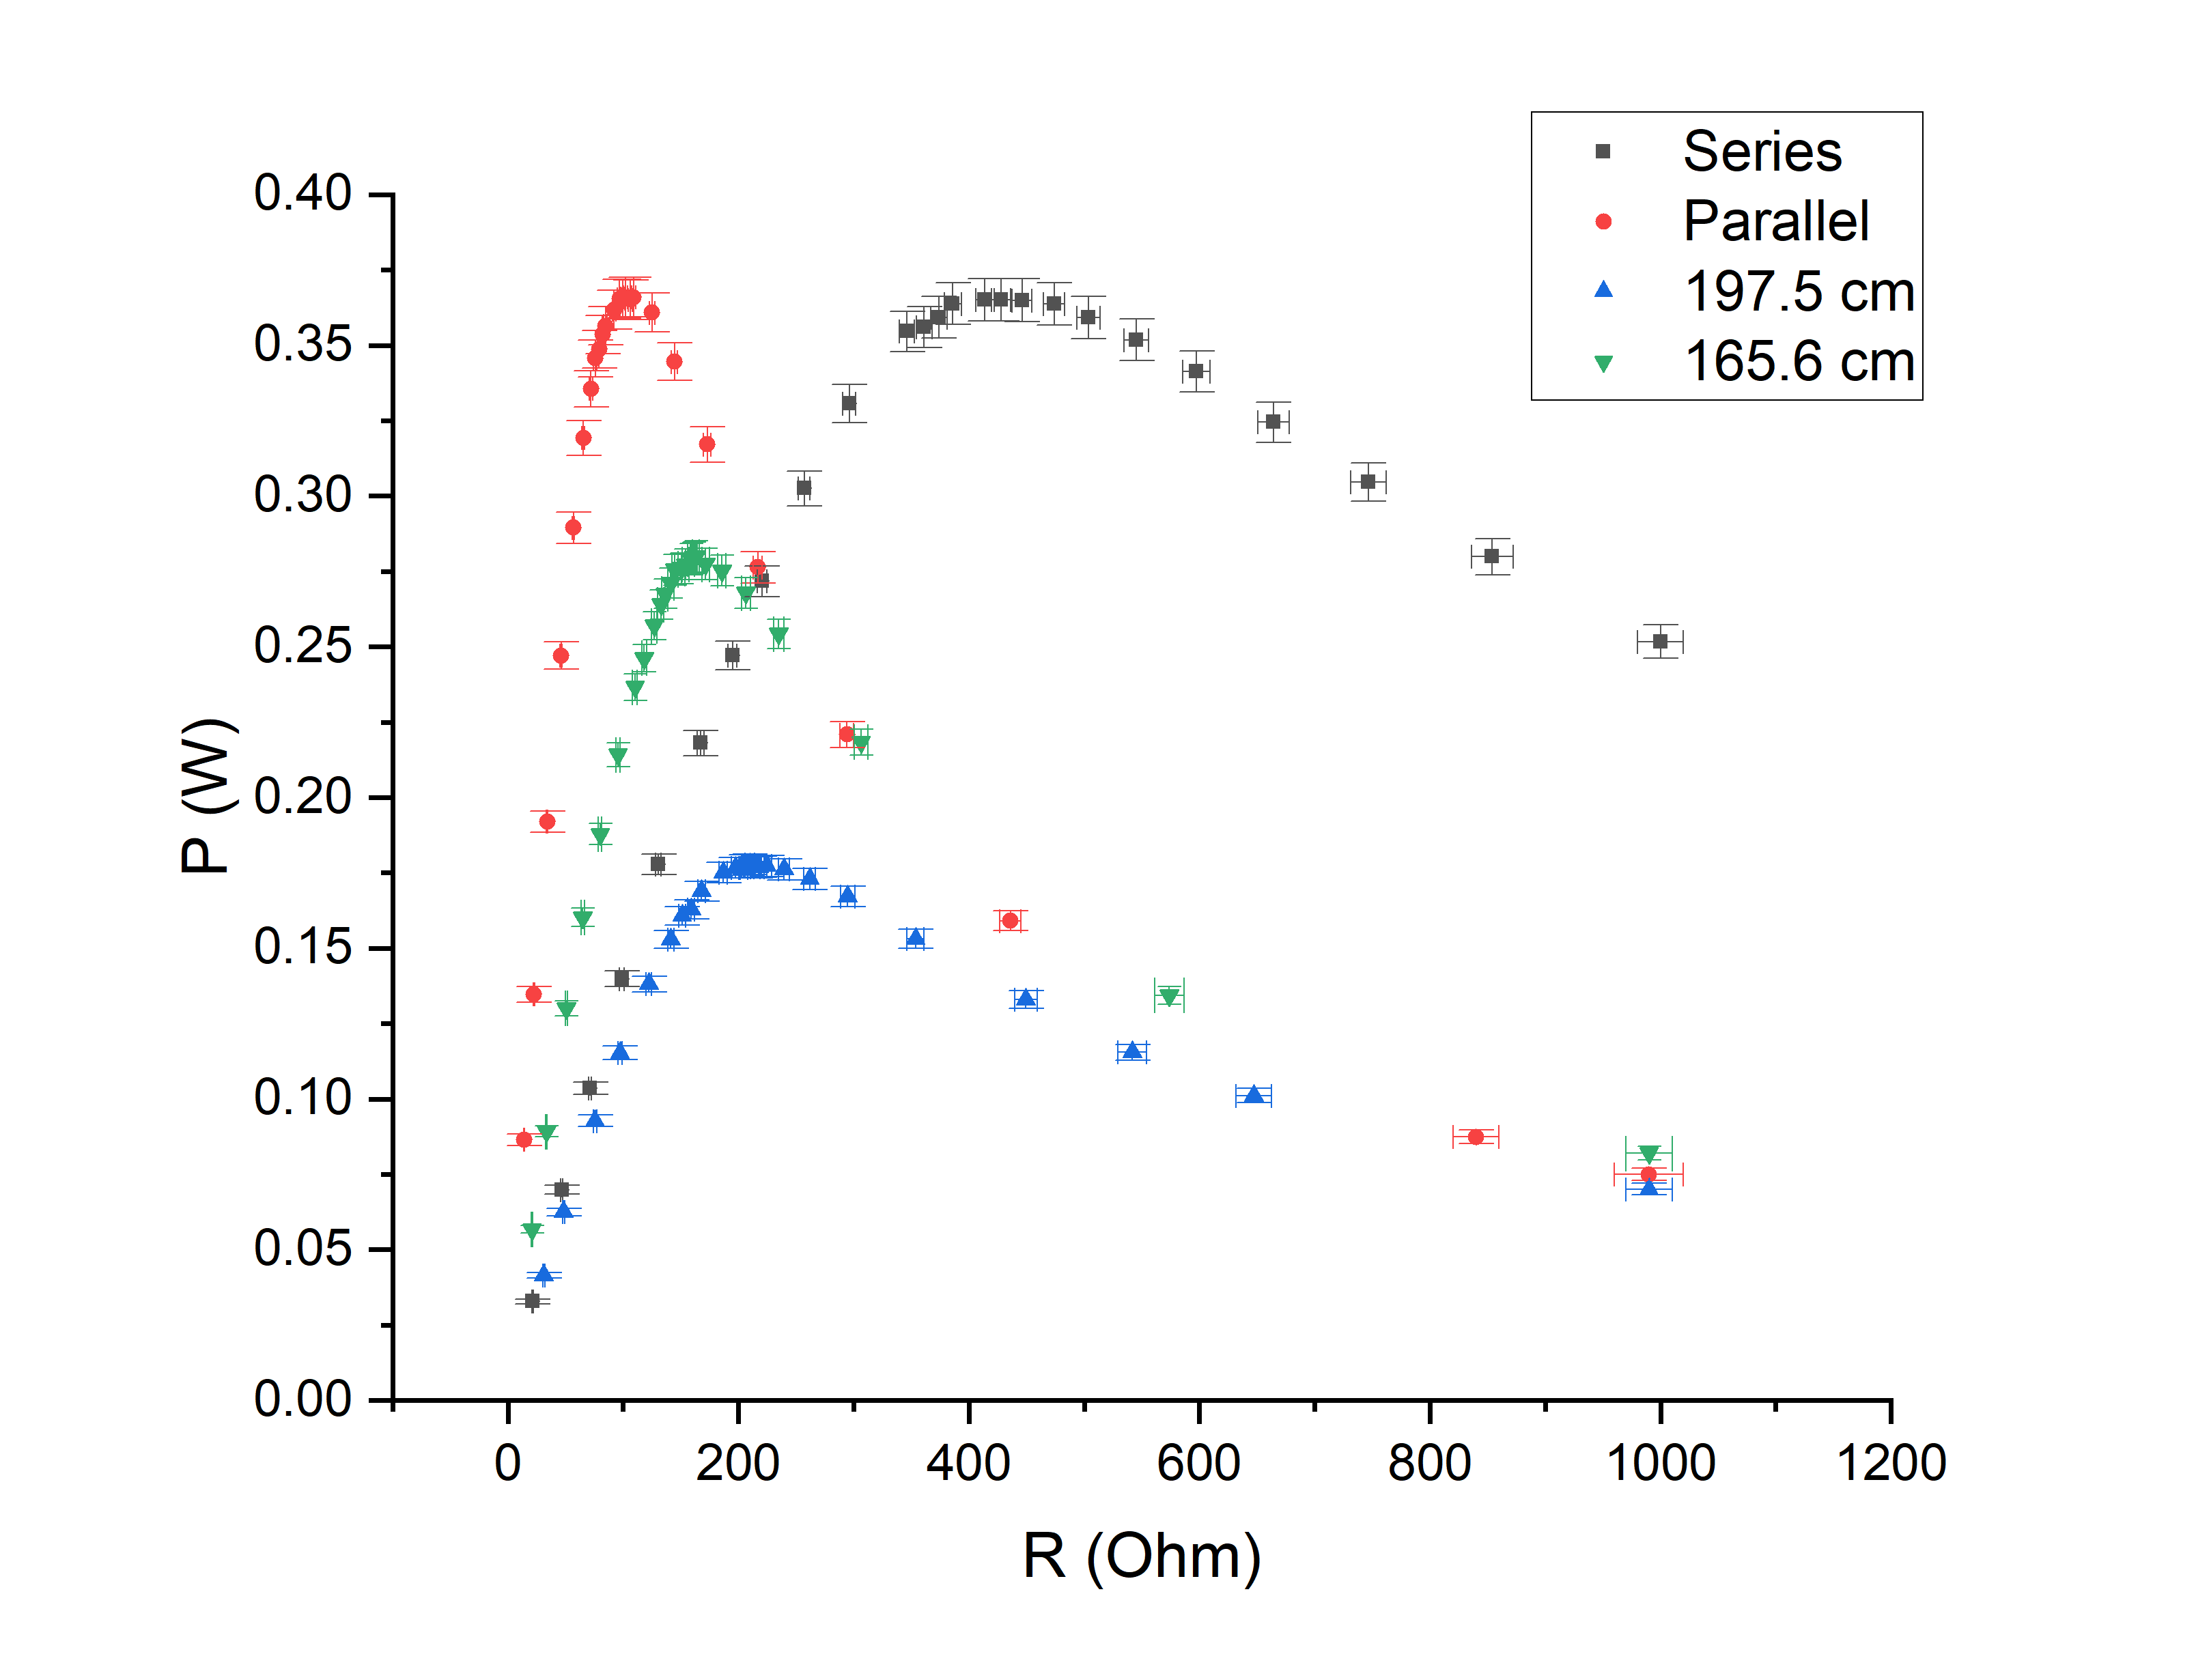
\includegraphics[scale=0.4]{R.png}
    \caption{$P$-$R$ characteristic curves of each configuration.}\label{FigR}
\end{figure}


\subsection{Maximum Output Power}

The maximum output power and the corresponding $V_\text{m}, I_\text{m}, R_\text{m}$ can be found by consulting Table 4 and 5. The results are presented in Table 6.

\begin{table}[H]\centering
    \begin{tabular}{ccccc}
        \toprule
                 & $V_\text{m}$ [V] & $I_\text{m}$ [mA] & $P_\text{m}$ [W]   & $R_\text{m}\,\,[\Omega]$ \\
        \midrule
        Series   & 12.29 $\pm$ 0.07 & 29.7 $\pm$ 0.5    & 0.365  $\pm$ 0.007 & 414   $\pm$ 8            \\
        Parallel & 6.12  $\pm$ 0.04 & 59.8 $\pm$ 1.0    & 0.366  $\pm$ 0.007 & 102.3 $\pm$ 1.8          \\
        197.5 cm & 6.11  $\pm$ 0.04 & 29.1 $\pm$ 0.5    & 0.178  $\pm$ 0.003 & 210   $\pm$ 4            \\
        165.6 cm & 6.76  $\pm$ 0.04 & 41.4 $\pm$ 0.7    & 0.280  $\pm$ 0.005 & 163   $\pm$ 3            \\
        \bottomrule
    \end{tabular}
    \caption{$V_\text{m}$, $I_\text{m}$ and $P_\text{m}$ in each configuration.}\label{tab:Pmax}
\end{table}

\subsection{Fill Factor (Single Configuration)}

To figure out the fill factor, $U_\text{oc}$ and $I_\text{sc}$ are measured. The data are shown in Table 7.

\begin{table}[H]
    \centering
    \begin{tabular}{ccc}
        \toprule
                 & $V_\text{oc}$ [V]  & $I_\text{sc}$ [mA] \\
        \midrule
        197.5 cm & 8.77    $\pm$ 0.05 & 37.2 $\pm$ 0.7     \\
        165.6 cm & 9.29    $\pm$ 0.06 & 52.9 $\pm$ 0.9     \\
        \bottomrule
    \end{tabular}
    \caption{Measurement data for $U_\text{oc}$ and $I_\text{sc}$.}\label{tab:ocsc}
\end{table}

The fill factor $FF$ can be then calculated out of Eq.1. Take the series configuration as an example,
$$FF = \frac{P_\text{m}}{V_\text{oc}I_\text{sc}} = \frac{0.178}{8.77\times 37.2\times 10^{-3}} = 0.545 \pm 0.015.$$

The fill factor of each single configuration are calculated as shown and the results are presented in Table 8.

\begin{table}[H]\centering
    \begin{tabular}{cc}
        \toprule
                 & $FF$               \\
        \midrule
        197.5 cm & 0.545  $\pm$ 0.015 \\
        165.6 cm & 0.569  $\pm$ 0.015 \\
        \bottomrule
    \end{tabular}
    \caption{Fill factor of single configuration.}\label{Tablefill}
\end{table}

\subsection{Energy Conversion Efficiency (Single Configuration)}

The measurement data for the area are shown in Table 9.
\begin{table}[H]\centering
    \begin{tabular}{cc}
        \toprule
        Length $L_1$ [cm] $\pm$ 0.1 [cm] & Width $L_2$ [cm] $\pm$ 0.1 [cm] \\
        \midrule
        26.0                             & 21.1                            \\
        \bottomrule
    \end{tabular}
    \caption{Measurement data for area.}\label{TableArea}
\end{table}

The measurement result of power of six points on the board are shown in Table 10.
\begin{table}[H]\centering
    \begin{tabular}{ccccccc}
        \toprule
                                                               & 1     & 2     & 3   & 4   & 5     & 6     \\
        \midrule
        $P_{197.5}\,\,[\text{W/m}^2] \pm 10\,\,[\text{W/m}^2]$ & 100.6 & 141.7 & 113 & 140 & 120.1 & 136.2 \\
        $P_{165.6}\,\,[\text{W/m}^2] \pm 10\,\,[\text{W/m}^2]$ & 157.3 & 178.5 & 166 & 185 & 189.5 & 188   \\
        \bottomrule
    \end{tabular}
    \caption{Measurement data for solar power.}\label{tab:Pin}
\end{table}

The average of the power per square meter is
$$\overline{P_{197.5}} = \frac{1}{6}(100.6 + 141.7 + 113 + 140 + 120.1 + 136.2) = (13 \pm 2)\times 10^1\,\,\text{W/m}^2,$$
$$\overline{P_{165.6}} = \frac{1}{6}(157.3 + 178.5 + 166 + 185 + 189.5 + 188) = (17.7 \pm 1.7)\times 10^1\,\,\text{W/m}^2.$$

The total power is
$$P_{\text{in},197.5} = \overline{P_{197.5}}L_1L_2 = 130 \times 0.260 \times 0.211 = 7.1 \pm 1.1\,\,\text{W},$$
$$P_{\text{in},165.6} = \overline{P_{165.6}}L_1L_2 = 177 \times 0.260 \times 0.211 = 9.7 \pm 0.9\,\,\text{W}.$$

The power energy conversion efficiency can then be calculated from Eq.2, as
$$\eta_{197.5} = \frac{P_\text{m}}{P_{\text{in},197.5}} \times 100\% = \frac{0.178}{7.13} \times 100\%= 2.5\% \pm 0.4\%,$$
$$\eta_{165.6} = \frac{P_\text{m}}{P_{\text{in},165.6}} \times 100\% = \frac{0.280}{9.71} \times 100\%= 2.9\% \pm 0.2\%,$$

\section{Conclusions and Discussion}

\subsection{$I$-$V$, $P$-$V$, $P$-$R$ Relation}

From Figure 2, we can see that $I$ decreases as the $V$ increases. Besides, its absolute value of the slope gets larger. This conforms to the characteristic if the diode in the solar sell.

From Figure 3 and 4, we can see that the as the $R$ (or $V$, since increase of $R$ will result in increase of $V$ according to Ohm's laws) increases, the power first increases and then decreases. The output power attains its maximum at some $R = R_m$. This agrees with the theoretical conclusions that are derived from the Ohm's laws.

\subsection{Parameters of the solar cell}

The parameters measured of the solar cell are summarized in Table 11. It can be seen that for $V_\text{m}$ and $V_\text{oc}$, the series is about twice of the single and the parallel is about equal to the single; for $I_\text{m}$ and $I_\text{sc}$, the series is about equal to the single and the parallel is about twice of the single. This conforms to the theoretical results.

Also, the fll factor and the energy conversion efficiency obtained also implies that the greater the fill factor, the greater the energy conversion efficiency. This verifies the idea stated in the Introduction part.

Furthermore, our results also implies that the closer the solar board is to the light source, that is, the greater the incident intensity, the greater the fill factor [2]. Also, the fill factor conforms to the fact that most solar cell is of fill factor 0.5$\sim$0.8 [2].

The energy conversion efficiency we obtained is rather low, which agrees with the fact that "traditional solar cell are of low efficiency" [3].


\begin{table}[H]\centering
    \begin{tabular}{ccccc}
        \toprule
                                 & Series             & Parallel          & 197.5 cm           & 165.6 cm          \\
        \midrule
        $V_\text{m}$ [V]         & 12.29 $\pm$ 0.07   & 6.12 $\pm$ 0.04   & 6.11 $\pm$ 0.04    & 6.76 $\pm$ 0.04   \\
        $I_\text{m}$ [mA]        & 29.7 $\pm$ 0.5     & 59.8 $\pm$ 1.0    & 29.1 $\pm$ 0.5     & 41.4 $\pm$ 0.7    \\
        $P_\text{m}$ [W]         & 0.365 $\pm$ 0.007  & 0.366 $\pm$ 0.007 & 0.178 $\pm$ 0.003  & 0.280 $\pm$ 0.005 \\
        $R_\text{m}\,\,[\Omega]$ & 414 $\pm$ 8        & 102.3 $\pm$ 1.8   & 210 $\pm$ 4        & 163 $\pm$ 3       \\
        $V_\text{oc}$ [V]        & 17.380 $\pm$ 0.010 & 8.83 $\pm$ 0.05   & 8.77 $\pm$ 0.05    & 9.29 $\pm$ 0.06   \\
        $I_\text{sc}$ [mA]       & 39.2 $\pm$ 0.7     & 80.1 $\pm$ 1.3    & 37.2 $\pm$ 0.7     & 52.90$\pm$ 0.9    \\
        $FF$                     & /                  & /                 & 0.545 $\pm$ 0.015  & 0.569 $\pm$ 0.015 \\
        $\eta$                   & /                  & /                 & $2.5\% \pm 0.4 \%$ & $2.9\% \pm 0.3\%$ \\
        \bottomrule
    \end{tabular}
    \caption{Results.}\label{TableResult}
\end{table}

\subsection{Causes for errors and uncertainties}

\begin{enumerate}
    \item Our movement during the measurement may affect the incident intensity.
    \item The input power of the solar cell is measured by choosing six points on the board, which can cause a huge uncertainty and further errors.
    \item The internal resistance of the solar cell may cause deviation from the theoretical conclusions, since it is assumed that the solar cell is of no internal resistance.
    \item The wire board we used has resistance itself, which caused the error in the experiment
    \item Only discrete data are obtained in our experiment. The maximum point is only the approximated one and may have a significant deviation from the real value.
    \item The loading resistance are obtained through the $V$-$I$ method. As is known, the method itself has systematic error.
\end{enumerate}

\subsection{Suggestions}

\begin{enumerate}
    \item Measure the loading resistance using a multimeter instead of using the $V$-$I$ method.
    \item Make the incident intensity less sensitive to the surroundings.
    \item Use apparatus with higher precision.
\end{enumerate}

\subsection{Conclusions}

To sum up, in this exercise, we got familiar with the working principle of a solar cell and studied the parameters and characteristic of the solar cell in different configuration. Some basic parameters are measured and calculated and characteristics of the solar cell are verified. The results all conforms to the theoretical values and conclusions.

\begin{thebibliography}{1}

    \bibitem{manual} VP241 Exercise 3: Solar Cells: $I$-$V$ Characteristics, UM-SJTU Joint Institude.
    \bibitem{website} https://doi.org/10.1016/0379-6787(83)90067-4
    \bibitem{website} https://www.worldscientific.com/doi/abs/10.1142/9781783264469\_0006

\end{thebibliography}

\newpage

\appendix

\section{Measurement Uncertainty Analysis}

\subsection{Uncertainty of $I$, $V$}
The uncertainty of $V$ is $0.5\%+0.01$ V, and the uncertainty of $I$ is $1.5\%+0.1$ mA. Take the first set of data as an example,
$$u_{V} = 0.5\% \times 0.84 + 0.01 = 0.01\,\text{V}.$$
$$u_{I} = 1.5\% \times 39.1 + 0.1 = 0.7\,\text{mA}.$$
All the uncertainties of $V$ and $I$ are calculated in this way and the results are shown in Table 12.

\begin{table}[H]\centering
    \begin{tabular}{ccc||cc||cc||cc}
        \toprule
           & \multicolumn{2}{c||}{Series} & \multicolumn{2}{c||}{Parallel} & \multicolumn{2}{c||}{197.5 cm} & \multicolumn{2}{c}{165.6 cm}                                                   \\
        \midrule
           & $u_V$ [V]                    & $u_I$ [mA]                     & $u_V$ [V]                      & $u_I$ [mA]                   & $u_V$ [V] & $u_I$ [mA] & $u_V$ [V] & $u_I$ [mA] \\
        \midrule
        1  & 0.01                         & 0.7                            & 0.02                           & 1.3                          & 0.02      & 0.6        & 0.02      & 0.9        \\
        2  & 0.02                         & 0.7                            & 0.02                           & 1.3                          & 0.02      & 0.6        & 0.02      & 0.9        \\
        3  & 0.02                         & 0.7                            & 0.02                           & 1.2                          & 0.02      & 0.6        & 0.02      & 0.9        \\
        4  & 0.03                         & 0.7                            & 0.03                           & 1.2                          & 0.03      & 0.6        & 0.03      & 0.8        \\
        5  & 0.03                         & 0.7                            & 0.03                           & 1.2                          & 0.03      & 0.6        & 0.03      & 0.8        \\
        6  & 0.04                         & 0.6                            & 0.03                           & 1.1                          & 0.03      & 0.6        & 0.03      & 0.8        \\
        7  & 0.04                         & 0.6                            & 0.03                           & 1.1                          & 0.03      & 0.6        & 0.04      & 0.8        \\
        8  & 0.05                         & 0.6                            & 0.04                           & 1.1                          & 0.04      & 0.6        & 0.04      & 0.8        \\
        9  & 0.05                         & 0.6                            & 0.04                           & 1.1                          & 0.04      & 0.6        & 0.04      & 0.8        \\
        10 & 0.06                         & 0.6                            & 0.04                           & 1.1                          & 0.04      & 0.6        & 0.04      & 0.8        \\
        11 & 0.07                         & 0.6                            & 0.04                           & 1.1                          & 0.04      & 0.5        & 0.04      & 0.8        \\
        12 & 0.07                         & 0.6                            & 0.04                           & 1.0                          & 0.04      & 0.5        & 0.04      & 0.8        \\
        13 & 0.07                         & 0.6                            & 0.04                           & 1.0                          & 0.04      & 0.5        & 0.04      & 0.8        \\
        14 & 0.07                         & 0.6                            & 0.04                           & 1.0                          & 0.04      & 0.5        & 0.04      & 0.7        \\
        15 & 0.07                         & 0.5                            & 0.04                           & 1.0                          & 0.04      & 0.5        & 0.04      & 0.7        \\
        16 & 0.07                         & 0.5                            & 0.04                           & 1.0                          & 0.04      & 0.5        & 0.04      & 0.7        \\
        17 & 0.07                         & 0.5                            & 0.04                           & 1.0                          & 0.04      & 0.5        & 0.04      & 0.7        \\
        18 & 0.08                         & 0.5                            & 0.04                           & 0.9                          & 0.04      & 0.5        & 0.04      & 0.7        \\
        19 & 0.08                         & 0.5                            & 0.05                           & 0.8                          & 0.04      & 0.5        & 0.04      & 0.7        \\
        20 & 0.08                         & 0.5                            & 0.05                           & 0.7                          & 0.05      & 0.5        & 0.05      & 0.7        \\
        21 & 0.08                         & 0.5                            & 0.05                           & 0.6                          & 0.05      & 0.4        & 0.05      & 0.6        \\
        22 & 0.08                         & 0.4                            & 0.05                           & 0.5                          & 0.05      & 0.4        & 0.05      & 0.6        \\
        23 & 0.09                         & 0.4                            & 0.05                           & 0.4                          & 0.05      & 0.3        & 0.05      & 0.5        \\
        24 & 0.09                         & 0.4                            & 0.05                           & 0.3                          & 0.05      & 0.3        & 0.05      & 0.3        \\
        25 & 0.09                         & 0.3                            & 0.05                           & 0.2                          & 0.05      & 0.2        & 0.06      & 0.2        \\
        \bottomrule
    \end{tabular}
    \caption{Uncertainty of the data for $I$-$V$ characteristic.}\label{TableUncIV}
\end{table}

\subsection{Uncertainty of $P$, $R$}

For $P = VI$, its uncertainty is calculated as
$$u_P = \sqrt{(\frac{\partial P}{\partial V}u_V)^2 + (\frac{\partial P}{\partial I}u_I)^2} = \sqrt{(Iu_V)^2 + (Vu_I)^2}.$$

For $R = \frac{V}{I}$, its uncertainty is calculated as
$$u_R = \sqrt{(\frac{\partial R}{\partial V}u_V)^2 + (\frac{\partial R}{\partial I}u_I)^2} = \sqrt{(\frac{u_V}{I})^2 + (-\frac{V}{I^2}u_I)^2}.$$

Take the first set of data as an example,
$$u_P = \sqrt{(Iu_V)^2 + (Vu_I)^2} = \sqrt{(39.1\times 10^{-3}\times 0.01)^2 + (0.84\times 0.7\times 10^{-3})^2} = 0.0008\,\text{W}.$$
$$u_R = \sqrt{(\frac{u_V}{I})^2 + (-\frac{V}{I^2}u_I)^2} = \sqrt{(\frac{0.01}{39.1\times 10^{-3}})^2 + (-\frac{0.84}{39.1^2}\times 0.7)^2} = 0.5\,\Omega .$$

The uncertainty of $P$ and $R$ of all data are calculated in this way and the results are shown in Table 13.

\begin{table}[H]\centering
    \begin{tabular}{ccc||cc||cc||cc}
        \toprule
           & \multicolumn{2}{c||}{Series} & \multicolumn{2}{c||}{Parallel} & \multicolumn{2}{c||}{197.5 cm} & \multicolumn{2}{c}{165.6 cm}                                                               \\
        \midrule
           & $u_P$ [W]                    & $u_R$ [$\Omega$]               & $u_P$ [W]                      & $u_R$ [$\Omega$]             & $u_P$ [W] & $u_R$ [$\Omega$] & $u_P$ [W] & $u_R$ [$\Omega$] \\
        \mi
        1  & 0.0008                       & 0.5                            & 0.0019                         & 0.3                          & 0.0009    & 0.7              & 0.0013    & 0.5              \\
        2  & 0.0014                       & 1.0                            & 0.003                          & 0.4                          & 0.0013    & 1.0              & 0.0018    & 0.7              \\
        3  & 0.002                        & 1.4                            & 0.004                          & 0.6                          & 0.0018    & 1.5              & 0.002     & 1.0              \\
        4  & 0.003                        & 1.9                            & 0.004                          & 0.8                          & 0.002     & 1.9              & 0.003     & 1.2              \\
        5  & 0.003                        & 2                              & 0.005                          & 1.0                          & 0.003     & 2                & 0.004     & 1.5              \\
        6  & 0.004                        & 3                              & 0.006                          & 1.2                          & 0.003     & 3                & 0.004     & 1.8              \\
        7  & 0.005                        & 4                              & 0.006                          & 1.3                          & 0.003     & 3                & 0.004     & 2                \\
        8  & 0.005                        & 4                              & 0.006                          & 1.4                          & 0.003     & 3                & 0.005     & 2                \\
        9  & 0.006                        & 5                              & 0.006                          & 1.4                          & 0.003     & 3                & 0.005     & 2                \\
        10 & 0.006                        & 6                              & 0.006                          & 1.5                          & 0.003     & 4                & 0.005     & 2                \\
        11 & 0.007                        & 7                              & 0.006                          & 1.5                          & 0.003     & 4                & 0.005     & 3                \\
        12 & 0.007                        & 7                              & 0.006                          & 1.7                          & 0.003     & 4                & 0.005     & 3                \\
        13 & 0.007                        & 7                              & 0.007                          & 1.7                          & 0.003     & 4                & 0.005     & 3                \\
        14 & 0.007                        & 7                              & 0.007                          & 1.8                          & 0.003     & 4                & 0.005     & 3                \\
        15 & 0.007                        & 8                              & 0.007                          & 1.8                          & 0.003     & 4                & 0.005     & 3                \\
        16 & 0.007                        & 8                              & 0.007                          & 1.9                          & 0.003     & 4                & 0.005     & 3                \\
        17 & 0.007                        & 9                              & 0.007                          & 2.0                          & 0.003     & 4                & 0.005     & 3                \\
        18 & 0.007                        & 9                              & 0.007                          & 2                            & 0.003     & 5                & 0.005     & 3                \\
        19 & 0.007                        & 10                             & 0.006                          & 3                            & 0.003     & 5                & 0.005     & 3                \\
        20 & 0.007                        & 11                             & 0.006                          & 3                            & 0.003     & 6                & 0.005     & 3                \\
        21 & 0.007                        & 12                             & 0.005                          & 4                            & 0.003     & 7                & 0.005     & 4                \\
        22 & 0.007                        & 14                             & 0.004                          & 6                            & 0.003     & 10               & 0.005     & 4                \\
        23 & 0.006                        & 15                             & 0.003                          & 9                            & 0.003     & 12               & 0.004     & 6                \\
        24 & 0.006                        & 18                             & 0.002                          & $2\times10^{1}$              & 0.002     & 15               & 0.003     & 13               \\
        25 & 0.006                        & $2\times10^{1}$                & 0.002                          & $3\times10^{1}$              & 0.0019    & $2\times10^{1}$  & 0.002     & $2\times10^{1}$  \\
        \bottomrule
    \end{tabular}
    \caption{Uncertainty of data for $P$ and $R$.}\label{TableUncPR}
\end{table}

\subsection{Uncertainty of Fill Factor (Single Configuration)}
The uncertainty of $V_\text{oc}$ and $I_\text{sc}$ is calulated in the same way as $V$ and $I$. The results are displayed in Table 14, together with the uncertainty of the maximum power.

\begin{table}[H]\centering
    \begin{tabular}{cccc}
        \toprule
                 & $u_{V_\text{oc}}$ [V] & $u_{I_\text{sc}}$ [mA] & $u_{P_\text{m}}$ [W] \\
        \midrule
        197.5 cm & 0.04                  & 0.5                    & 0.003                \\
        165.6 cm & 0.04                  & 0.7                    & 0.005                \\
        \bottomrule
    \end{tabular}
    \caption{Uncertainty of $V_\text{oc}$ and $I_\text{sc}$.}
    \label{tab:uncocsc}
\end{table}

The uncertainty of fill factor, $FF = P_\text{m}/(V_\text{oc}I_\text{sc})$, is calculated as
\begin{align*}
    u_{FF} & = \sqrt{(\frac{\partial FF}{\partial P_\text{m}}u_{P_\text{m}})^2 + (\frac{\partial FF}{\partial V_\text{oc}}u_{V_\text{oc}})^2 + (\frac{\partial FF}{\partial I_\text{sc}}u_{I_\text{sc}})^2}   \\
           & = \sqrt{(\frac{1}{V_\text{oc}I_\text{sc}}u_{P_\text{m}})^2 + (-\frac{P_\text{m}}{V_\text{oc}^2I_\text{sc}}u_{V_\text{oc}})^2 + (-\frac{P_\text{m}}{V_\text{oc}I_\text{sc}^2}u_{I_\text{sc}})^2},
\end{align*}

Take the first set of data as an example,
\begin{align*}
    u_{FF} & = \sqrt{(\frac{1}{V_\text{oc}I_\text{sc}}u_{P_\text{m}})^2 + (-\frac{P_\text{m}}{V_\text{oc}^2I_\text{sc}}u_{V_\text{oc}})^2 + (-\frac{P_\text{m}}{V_\text{oc}I_\text{sc}^2}u_{I_\text{sc}})^2}      \\
           & = \sqrt{(\frac{1}{8.77\times 37.2\times 10^{-3}}\times 0.003)^2 + (-\frac{0.178}{8.77^2\times 37.2\times 10^{-3}}\times 0.05)^2 + (-\frac{0.178}{8.77\times (37.2\times 10^{-3})^2}\times 0.0007)^2} \\
           & = 0.015.
\end{align*}

The uncertainties are calculated as shown above and the results are shown in Table 15.

\begin{table}[H]\centering
    \begin{tabular}{cc}
        \toprule
                 & $u_{FF}$ \\
        \midrule
        197.5 cm & 0.015    \\
        165.6 cm & 0.015    \\
        \bottomrule
    \end{tabular}
    \caption{Uncertainty of $FF$.}\label{tab:uncFF}
\end{table}

\subsection{Uncertainty of Energy Conversion Efficiency (Single Configuration)}
The type--$B$ uncertainty of power measurement is $u_{P} = \Delta_{P,B} = \Delta_{dev} = 10\,\,[\text{W/m}^2]$. Since the power measurement is repeated for 6 times, the type--$A$ uncertainty needs to be considered.

In this case, $n$ = 6, $t_{0.95} = 2.57$, the type–-$A$ uncertainty is
\begin{align*}
    \Delta_{P,A} = & \frac{t_{0.95}}{\sqrt{n}} s_{\overline{P}}                                                \\
    =              & \frac{t_{0.95}}{\sqrt{n}} \sqrt{\frac{1}{n-1}\sum \limits_{i=1}^{n}(P _i-\overline{P})^2} \\
    =              & \frac{2.57}{\sqrt{6}}\sqrt{\frac{1}{6-1}\sum \limits_{i=1}^{6}(P_i-\overline{P})^2}.
\end{align*}

The total uncertainty is then
$$u_{\overline{P}} = \sqrt{\Delta_{P,A}^2+\Delta_{P,B}^2} = \sqrt{\bigg(\frac{2.57}{\sqrt{6}}\sqrt{\frac{1}{6-1}\sum \limits_{i=1}^{6}(P_i-\overline{P})^2}\bigg)^2+10^2}.$$

Hence, for the two single configurations,
$$u_{\overline{P_{197.5}}} = \sqrt{\bigg(\frac{2.57}{\sqrt{6}}\sqrt{\frac{1}{6-1}\sum \limits_{i=1}^{6}(P_i-125.27)^2}\bigg)^2+10^2} = 2.0\times 10^1\,\,\text{W/m}^2,$$
$$u_{\overline{P_{165.6}}} = \sqrt{\bigg(\frac{2.57}{\sqrt{6}}\sqrt{\frac{1}{6-1}\sum \limits_{i=1}^{6}(P_i-177.38)^2}\bigg)^2+10^2} = 1.7\times 10^1\,\,\text{W/m}^2,$$

The uncertainty of $P_\text{in} = \overline{P}L_1L_2$ is calculated as
\begin{align*}
    u_{P_\text{in}} & = \sqrt{(\frac{\partial P_{\text{in}}}{\partial \overline{P}}u_{\overline{P}})^2 + (\frac{\partial P_{\text{in}}}{\partial L_1}u_{L_1})^2 + (\frac{\partial P_\text{in}}{\partial L_2}u_{L_2})^2} \\
                    & = \sqrt{(L_1L_2u_{\overline{P}})^2 + (\overline{P}L_2u_{L_1})^2 + (\overline{P}L_1u_{L_2})^2}.
\end{align*}

Hence, substituting the values, it can be obtained that
$$u_{P_{\text{in},197.5}} = 1.1\,\,\text{W},\hspace{2em}u_{P_{\text{in},165.6}} = 0.9\,\,\text{W}.$$

Finally, the uncertainty of $\eta = (P_{\text{m}}/P_\text{in})\times 100\%$ can be calculated, as
\begin{align*}
    u_\eta & = \sqrt{(\frac{\partial \eta}{\partial P_\text{m}}u_{P_\text{m}})^2 + (\frac{\partial \eta}{\partial P_\text{in}}u_{P_\text{in}})^2} \times 100\% \\
           & = \sqrt{(\frac{1}{P_\text{in}}u_{P_\text{m}})^2 + (-\frac{P_{\text{m}}}{P_{\text{in}}^2}u_{P_\text{in}})^2} \times 100\%.
\end{align*}

Substituting the values, it is derived in the end that
$$u_{\eta_{197.5}} = 0.4\,\%,\hspace{2em}u_{\eta_{165.6}} = 0.2\,\%.$$

\section{Data Sheet}
Please find the original data sheet at the end of this report.

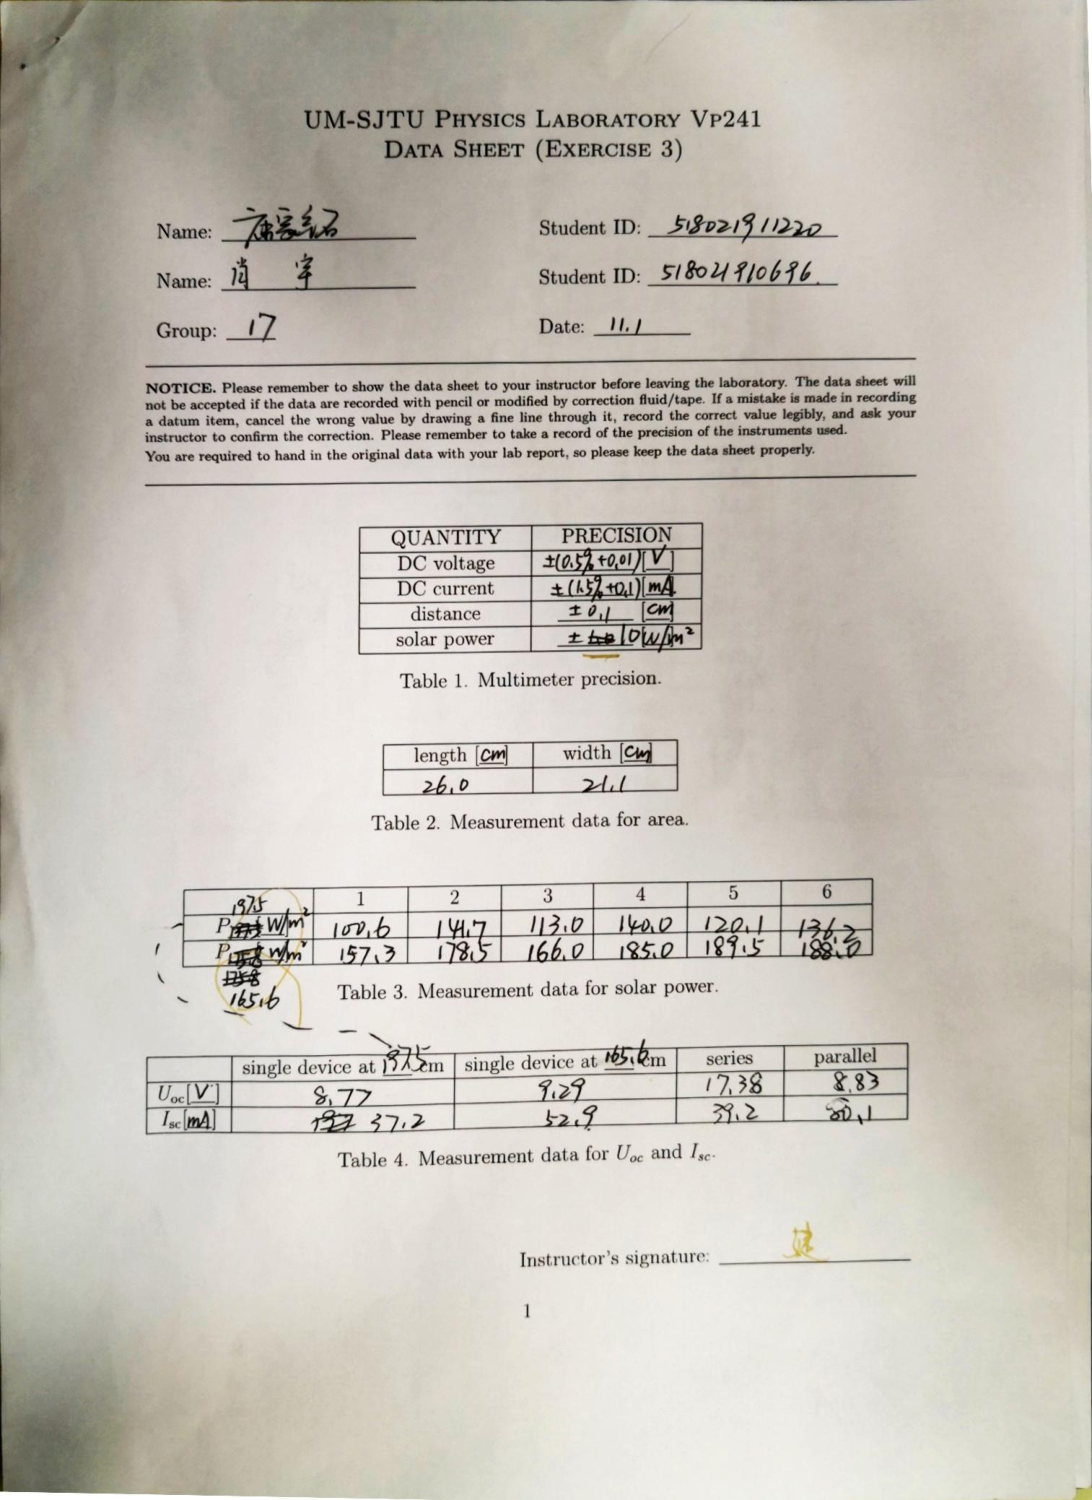
\includepdf[pages=-]{lab3datasheet.pdf}

\end{document}